\chapter{Tests}

\section{Schematics}

float barrier command to ensure that text stays close to the picture but no text from after the picture.

\subsection{part 1}

\begin{figure}[ht]
    \centering
    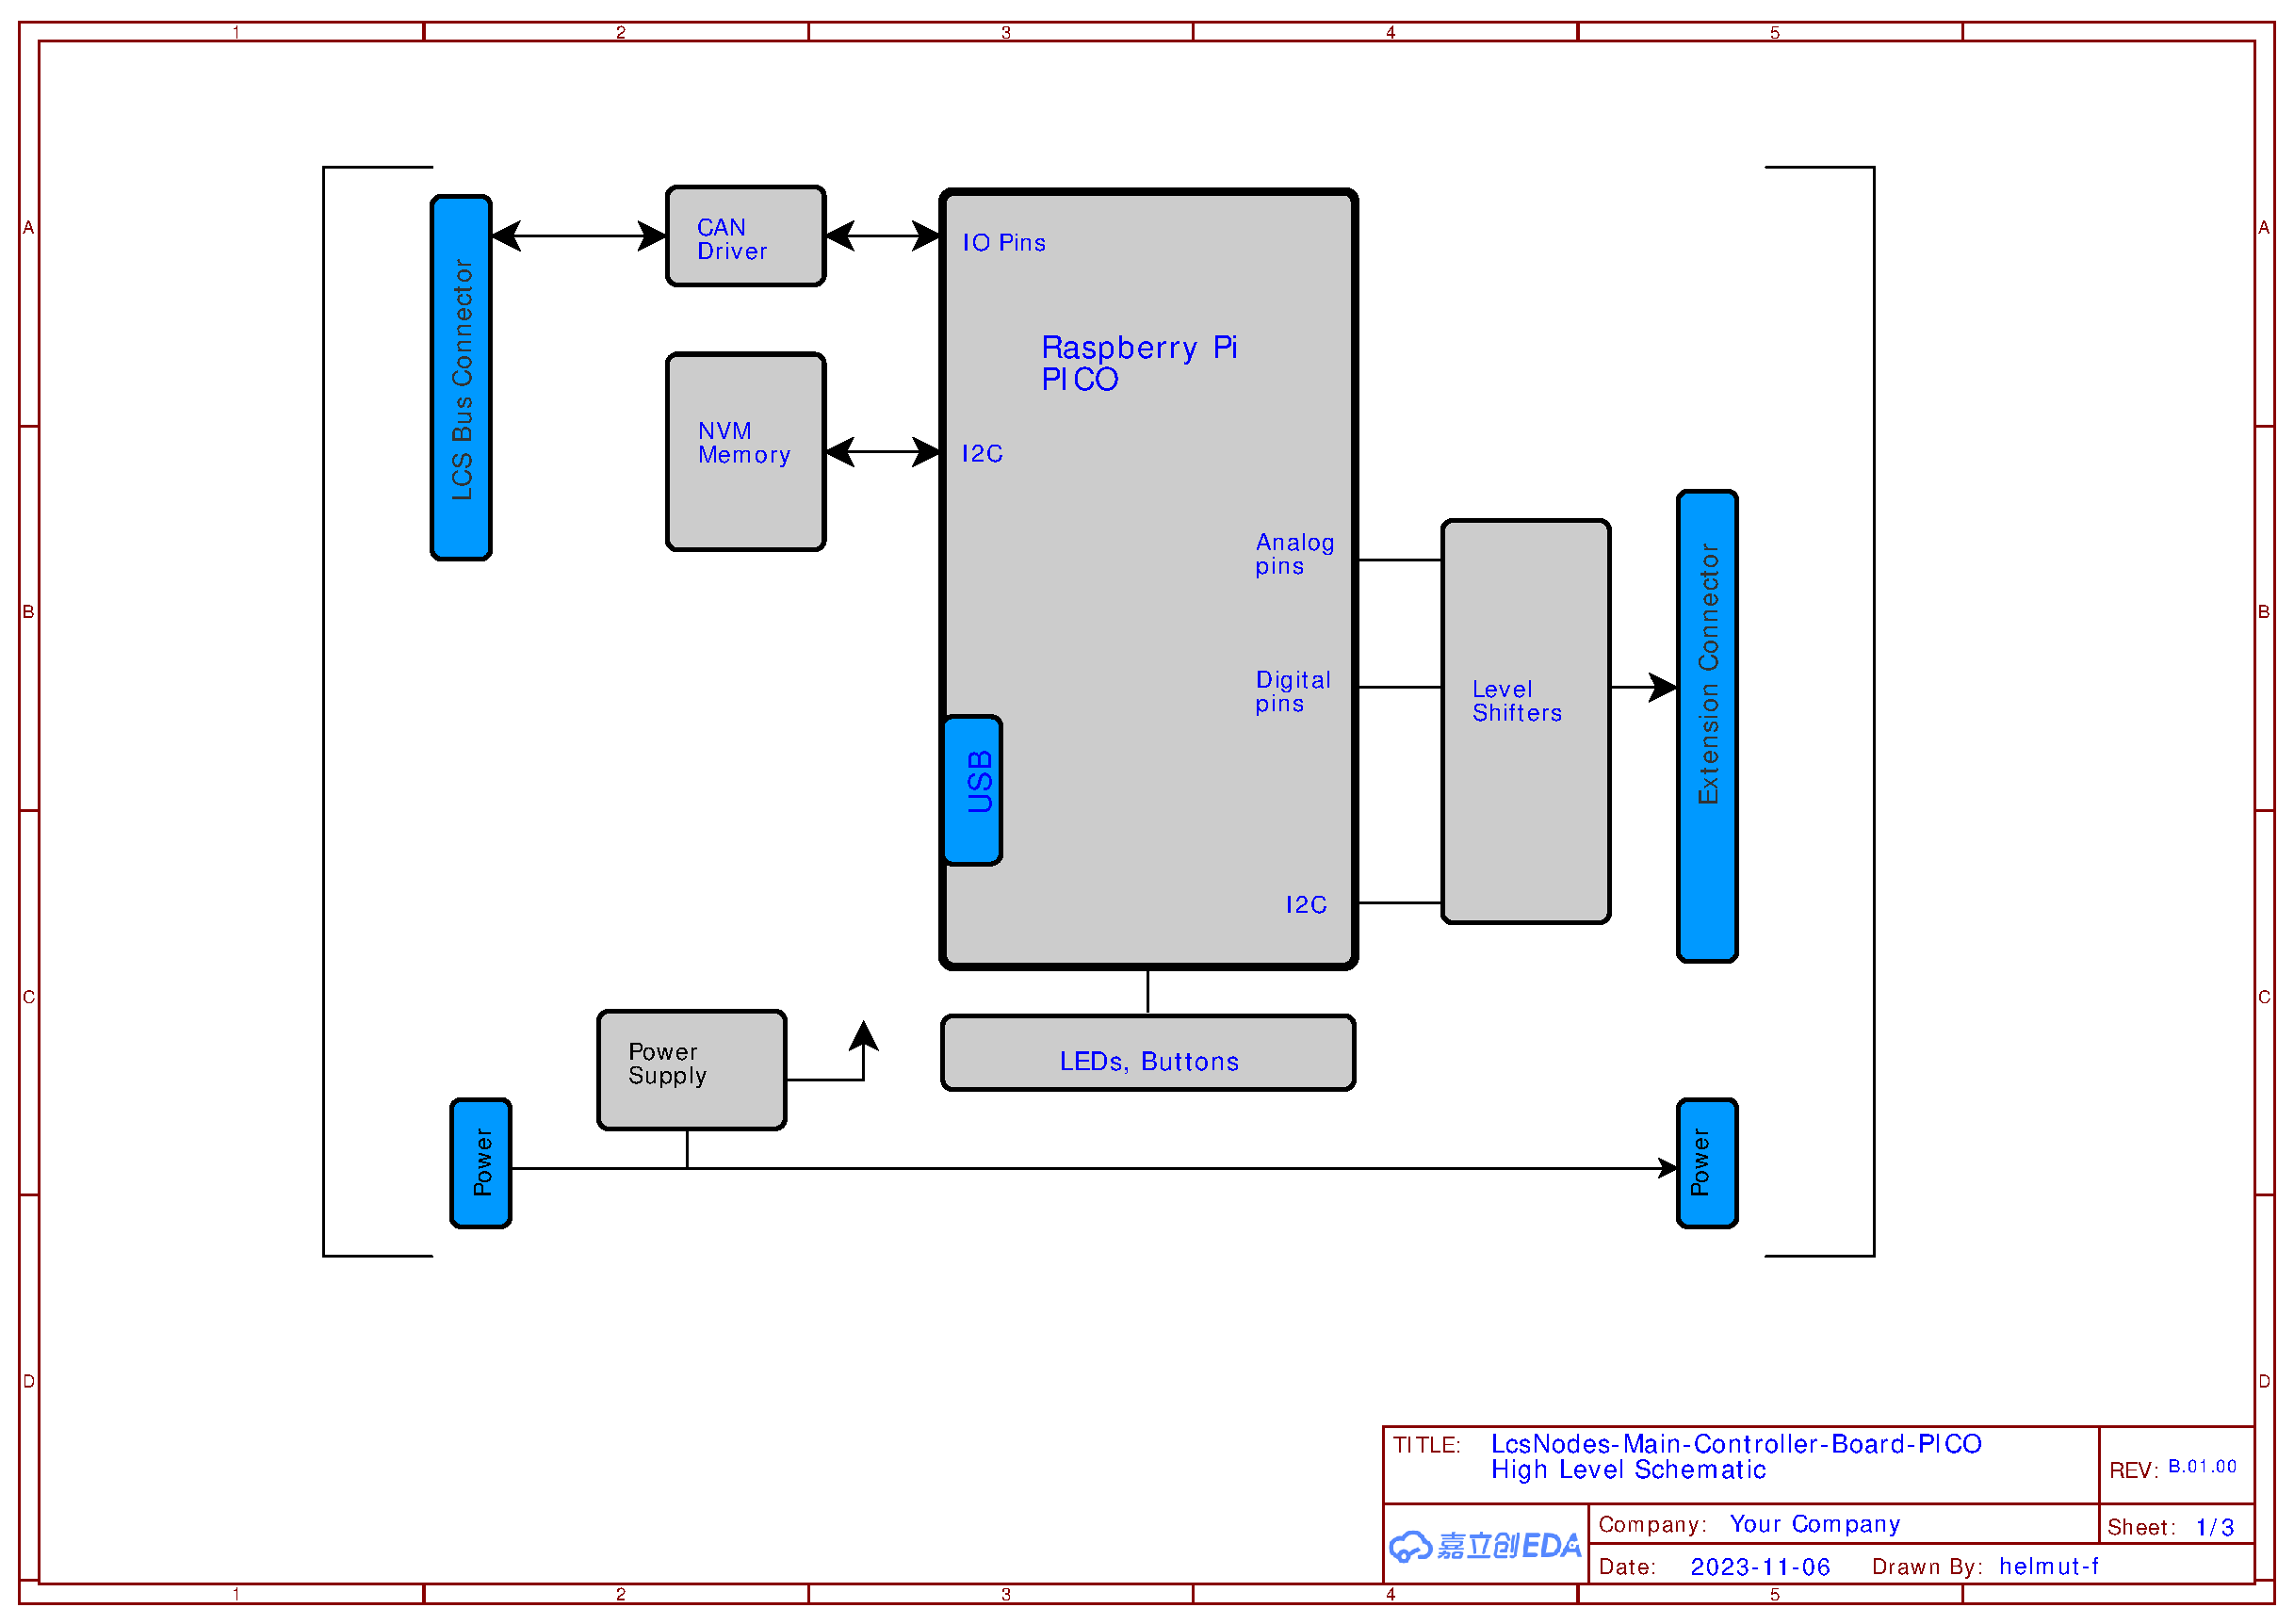
\includegraphics[page=1, width=\textwidth]{./schematics/Schematic_LcsNodes-Main-Controller-Board.pdf}
\end{figure}

\FloatBarrier

\subsection{part 2}
\begin{figure}[ht]
    \centering
    \includegraphics[page=2, width=\textwidth]{./schematics/Schematic_LcsNodes-Main-Controller-Board.pdf}
\end{figure}

\FloatBarrier

\subsection{part 3}
\begin{figure}[ht]
    \centering
    \includegraphics[page=3, width=\textwidth]{./schematics/Schematic_LcsNodes-Main-Controller-Board.pdf}
\end{figure}

\FloatBarrier


\section{Lists}

\subsection{A simple list}

\begin{itemize}
    \item First bullet point
    \item Second bullet point
    \item Third bullet point
\end{itemize}



\subsection{An instruction word layout}

A little test for an instruction word layout ... will be a bit fiddling work ... 

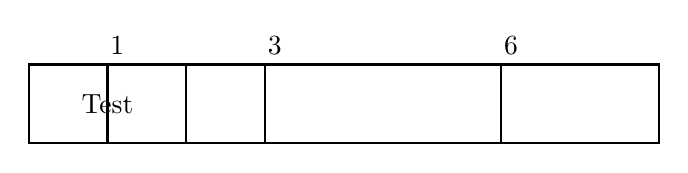
\begin{tikzpicture}
    \draw[thick] (0, 0) rectangle (8, 1); % Simple rectangle
    \node at (1, 0.5) {Test};   % Centered text
    \draw[thick] (2, 0) -- (2, 1);

    \foreach \x in {1, 3, 6} {
        \draw[thick] (\x, 0) -- (\x, 1); % Vertical line
        \node[above] at (\x + 0.125, 1) {\x}; % a number above the field
    }

\end{tikzpicture}


% example for the protocol chapter... instead of the tables....

\section{Protocol boxes}

A bit cumbersome and we would need to have text at defined locations. Perhaps keep the simple table in the protocol chapter.




\begin{center}
\begin{tikzpicture}

    \draw[help lines, gray!50, dashed] (0,0) grid( 16,8);

    \node[  draw, 
            rectangle, 
            minimum width=6cm, 
            minimum height=4cm, 
            text height=1cm, 
            align=left] (A) at (4, 4) 
            { };

    \node[  draw, 
            rectangle, 
            minimum width=6cm, 
            minimum height=4cm, 
            text height=1cm, 
            align=left] (B) at (12, 4) 
            { };

    \draw[->] (A.north east) ++(0, -1) -- ($(B.west) + (0, 1 )$);
    \draw[->] (B.south west) ++(0,  1) -- ($(A.east) + (0, -1)$);

    \node at ( 4,  6.25 ) {\textbf{Node A}};
    \node at ( 12, 6.25 ) {\textbf{Node B}};

    \node at ( 2.25,  5 ) {\textbf{LCS\_TOF}};
    \node at ( 10.25, 3 ) {\textbf{LCS\_TOF}};

\end{tikzpicture}
\end{center}



\section{Split rectangle}

We would need the split rectangle for the runtime area maps....

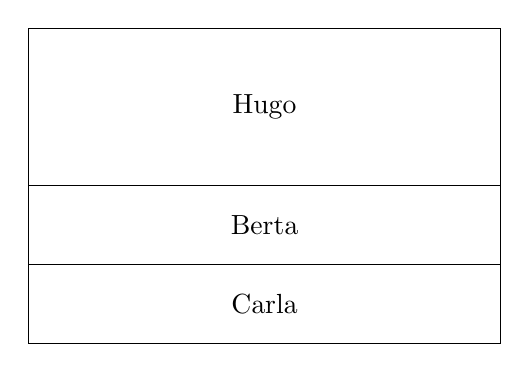
\begin{tikzpicture}

    \draw[draw](0,0) rectangle (6,4);
    \draw[draw](0,2) -- (6,2);
    \draw[draw](0,1) -- (6,1);

    \node at (3, 3.0) {Hugo};
    \node at (3, 1.5) {Berta};
    \node at (3, 0.5) {Carla};
\end{tikzpicture}

\section{Using tikzstyle}

Another test with tikzstyle. It still is a lot of work to even make simple pictures look nice :-)

\begin{tikzpicture}
    \draw[help lines, gray!50, dashed] (0,0) grid(16,12);

    % Thick horizontal line (LCS bus) with text
    \draw[line width=1.5mm, <->, line cap=round, draw=gray, name path=lcsline] 
        (0,8) -- (16,8)
        node[pos= 0.9, tsLargeBold, below] {LCS bus};

    % Define nodes
    \node[  tsRoundedRectangle, 
            minimum width=3cm,
            minimum height=1.5cm,
            text width=3cm,
            text centered,
            fill=red!50] (gw) at (3,10) {Gateways};

    \node[  tsRoundedRectangle, 
            minimum width=3cm,
            minimum height=1.5cm,
            text width=3cm,
            text centered,
            fill=red!50] (bs) at (7,10) {Base\\Station};

    \node[  tsRoundedRectangle, 
            minimum width=3cm,
            minimum height=1.5cm,
            text width=3cm,
            text centered,
            fill=red!50] (ch) at (13,10) {Cab\\Handheld};

    % Connecting arrows to LCS bus
    \path[name path=p1] (gw.south) -- (3,8); % Define arrow path
    \path[name intersections={of=lcsline and p1, by=intpoint1}];
    \coordinate (adjustedPoint1) at ($(intpoint1) + (0,0.75mm)$);
    \draw[<->, ultra thick, line cap=round] (gw.south) -- (adjustedPoint1);

    % Arrow from Base Station
    \path[name path=p2] (bs.south) -- (7,8); % Define arrow path
    \path[name intersections={of=lcsline and p2, by=intpoint2}]; % Find intersection
    \coordinate (adjustedPoint2) at ($(intpoint2) + (0,0.75mm)$);
    \draw[<->, ultra thick, line cap=round] (bs.south) -- (adjustedPoint2); % Draw to intersection

    % Arrow from Cab Handheld
    \path[name path=p3] (ch.south) -- (13,8);
    \path[name intersections={of=lcsline and p3, by=intpoint3}];
    \coordinate (adjustedPoint3) at ($(intpoint3) + (0,0.75mm)$);
    \draw[<->, ultra thick, line cap=round] (ch.south) -- (adjustedPoint3);

    % Other nodes
    \node[  tsRoundedRectangle,  
            minimum width=3cm,
            minimum height=1.5cm,
            text width=3cm,
            text centered,
            fill=red!50] (bc) at (4,6) {Block\\Controller};

    \node[  tsRoundedRectangle, 
            minimum width=3cm,
            minimum height=1.5cm,
            text centered,
            text width=3cm, fill=red!50] (s) at (8,6) {Sensors};

    \node[  tsRoundedRectangle, 
            minimum width=3cm,
            minimum height=1.5cm,
            text width=3cm,
            text centered, 
            fill=red!50] (a) at (12,6) {Actors};

    % Vertical arrows to LCS bus \path[name path=p3] (bc.north) -- (4,8);
    \path[name path=p4] (bc.north) -- (4,8);
    \path[name intersections={of=lcsline and p4, by=intpoint4}];
    \coordinate (adjustedPoint4) at ($(intpoint4) - (0,0.75mm)$);
    \draw[<->, ultra thick, line cap=round] (bc.north) -- (adjustedPoint4);

    \path[name path=p5] (s.north) -- (8,8);
    \path[name intersections={of=lcsline and p5, by=intpoint5}];
    \coordinate (adjustedPoint5) at ($(intpoint5) - (0,0.75mm)$);
    \draw[<->, ultra thick, line cap=round] (s.north) -- (adjustedPoint5);

    \path[name path=p6] (a.north) -- (12,8);
    \path[name intersections={of=lcsline and p6, by=intpoint6}];
    \coordinate (adjustedPoint6) at ($(intpoint6) - (0,0.75mm)$);
    \draw[<->, ultra thick, line cap=round] (a.north) -- (adjustedPoint6);

    % Ellipses with connections
    \node[  tsEllipse, 
            minimum width=3cm,
            minimum height=1.5cm,
            text width=3cm,
            text centered,
            fill=green!70] at (4,2) (blk) {Layout\\Blocks};

    \node[  tsEllipse, 
            minimum width=3cm,
            minimum height=1.5cm,
            text width=3cm,
            text centered,
            fill=green!70] at (10,2) (le) {Layout\\Elements};

    \draw[<->, ultra thick, line cap=round] (bc.south) -- (blk.north);
    \draw[<->, ultra thick, line cap=round] (s.south) -- ($(le.north) - (0.4,0)$);
    \draw[<->, ultra thick, line cap=round] (a.south) -- ($(le.north) + (0.4,0)$);
\end{tikzpicture}













\begin{tikzpicture}
    \draw[help lines, gray!50, dashed] (0,0) grid(16,12);

  
    % Define nodes
    \node[  tsRoundedRectangle, 
            minimum width=12cm,
            minimum height=1.5cm,
            text width=3cm,
            text centered,
            fill=red!50] (fl) at (8,10) {Firmware Layer};

    \node[  tsRoundedRectangle, 
            minimum width=3cm,
            minimum height=1.5cm,
            text width=3cm,
            text centered,
            fill=red!50] (rl) at (8,7) {LCS Runtime Library};

    \node[  tsRoundedRectangle, 
            minimum width=3cm,
            minimum height=1.5cm,
            text width=3cm,
            text centered,
            fill=red!50] (mh) at (13,10) {Module Hardware};

    % Connecting arrows to LCS bus
    %\path[name path=p1] (gw.south) -- (3,8); % Define arrow path
    %\path[name intersections={of=lcsline and p1, by=intpoint1}];
    %\coordinate (adjustedPoint1) at ($(intpoint1) + (0,0.75mm)$);
    %\draw[<->, ultra thick, line cap=round] (gw.south) -- (adjustedPoint1);

    % Arrow from Base Station
    %\path[name path=p2] (bs.south) -- (7,8); % Define arrow path
    %\path[name intersections={of=lcsline and p2, by=intpoint2}]; % Find intersection
    %\coordinate (adjustedPoint2) at ($(intpoint2) + (0,0.75mm)$);
    %\draw[<->, ultra thick, line cap=round] (bs.south) -- (adjustedPoint2); % Draw to intersection

    % Arrow from Cab Handheld
    %\path[name path=p3] (ch.south) -- (13,8);
    %\path[name intersections={of=lcsline and p3, by=intpoint3}];
    %\coordinate (adjustedPoint3) at ($(intpoint3) + (0,0.75mm)$);
    %\draw[<->, ultra thick, line cap=round] (ch.south) -- (adjustedPoint3);


   
   % \draw[<->, ultra thick, line cap=round] (bc.south) -- (blk.north);
   % \draw[<->, ultra thick, line cap=round] (s.south) -- ($(le.north) - (0.4,0)$);
   % \draw[<->, ultra thick, line cap=round] (a.south) -- ($(le.north) + (0.4,0)$);
\end{tikzpicture}


